\documentclass[a4paper,12pt,ngerman]{scrartcl}

% Language
\usepackage{polyglossia}
\setmainlanguage{german}

% Grafiken
\usepackage{graphicx}

% Make \today print in format "NN<st|nd|rd|th> MM YYYY"
\usepackage{isodate}
\origdate

\linespread{1.15}

% Titel anders formatieren mit: Command, Format, Label, Sep, Before-Code
\usepackage{titlesec}
\titleformat{\section}{\sffamily\Large\bfseries}{}{0pt}{}
\titleformat{\subsection}{\sffamily\large\bfseries}{}{0pt}{}

% Own pagestyle (header and footer)
\usepackage{fancyhdr}
\fancyhf{} % Clear header and footer content
\fancyhead[L]{{\small \textsf{WS 14/15, Informationsvisualisierung}}}
\fancyhead[C]{{\small \textsf{Übung 4}}}
\fancyhead[R]{{\small \textsf{\today}}}
\fancyfoot[C]{\thepage}

% Text in quotes
% Usage: \enquote{To be or not to be.}
\usepackage{csquotes}

% Subliminal refinements towards typographical perfection
\usepackage{microtype}

% Footnotes in section
\usepackage[stable]{footmisc}

% Better refs with \cref{}
\usepackage[capitalize,noabbrev]{cleveref}

% Borders
\usepackage[paper=a4paper,left=20mm,right=20mm,top=30mm,bottom=30mm]{geometry}

\usepackage{longtable}

\begin{document}
\pagestyle{fancy} % Activate own pagestyle

\section{Aufgabe 4.1 | Treemaps}
\subsection*{Slice-And-Dice}

Der Slice-And-Dice-Algorithmus schafft auf eine relativ einfache Art und Weise eine übersichtliche TreeMap. Zunächst wird die Grundfläche entlang einer Achse in so viele Rechtecke geteilt, wie die Wurzel Kinder hat. Die Größe eines Rechtecks entspricht dabei immer der "Größe" des jeweiligen Kindes, die sich durch die Summe aller ihm untergeordneten Blätter errechnet (sofern es nicht selbst ein Blatt ist). Im nächsten Schritt werden dann die Kindeskinder nach dem gleichen Verfahren in der Fläche des entsprechenden Kindes verteilt, wobei die Partitionierung diesmal entlang der anderen Achse durchgeführt wird. So wird weiter verfahren bis alle Blätter erreicht sind (Breitensuche), wichtig ist dabei, dass in jedem Schritt die Achse gewechselt wird, nach der die Partitionierung stattfindet. Das Ergebnis für den gegebenen Baum zeigt \cref{fig:sliceAndDice}.

\begin{figure}[ht]
    \centering
    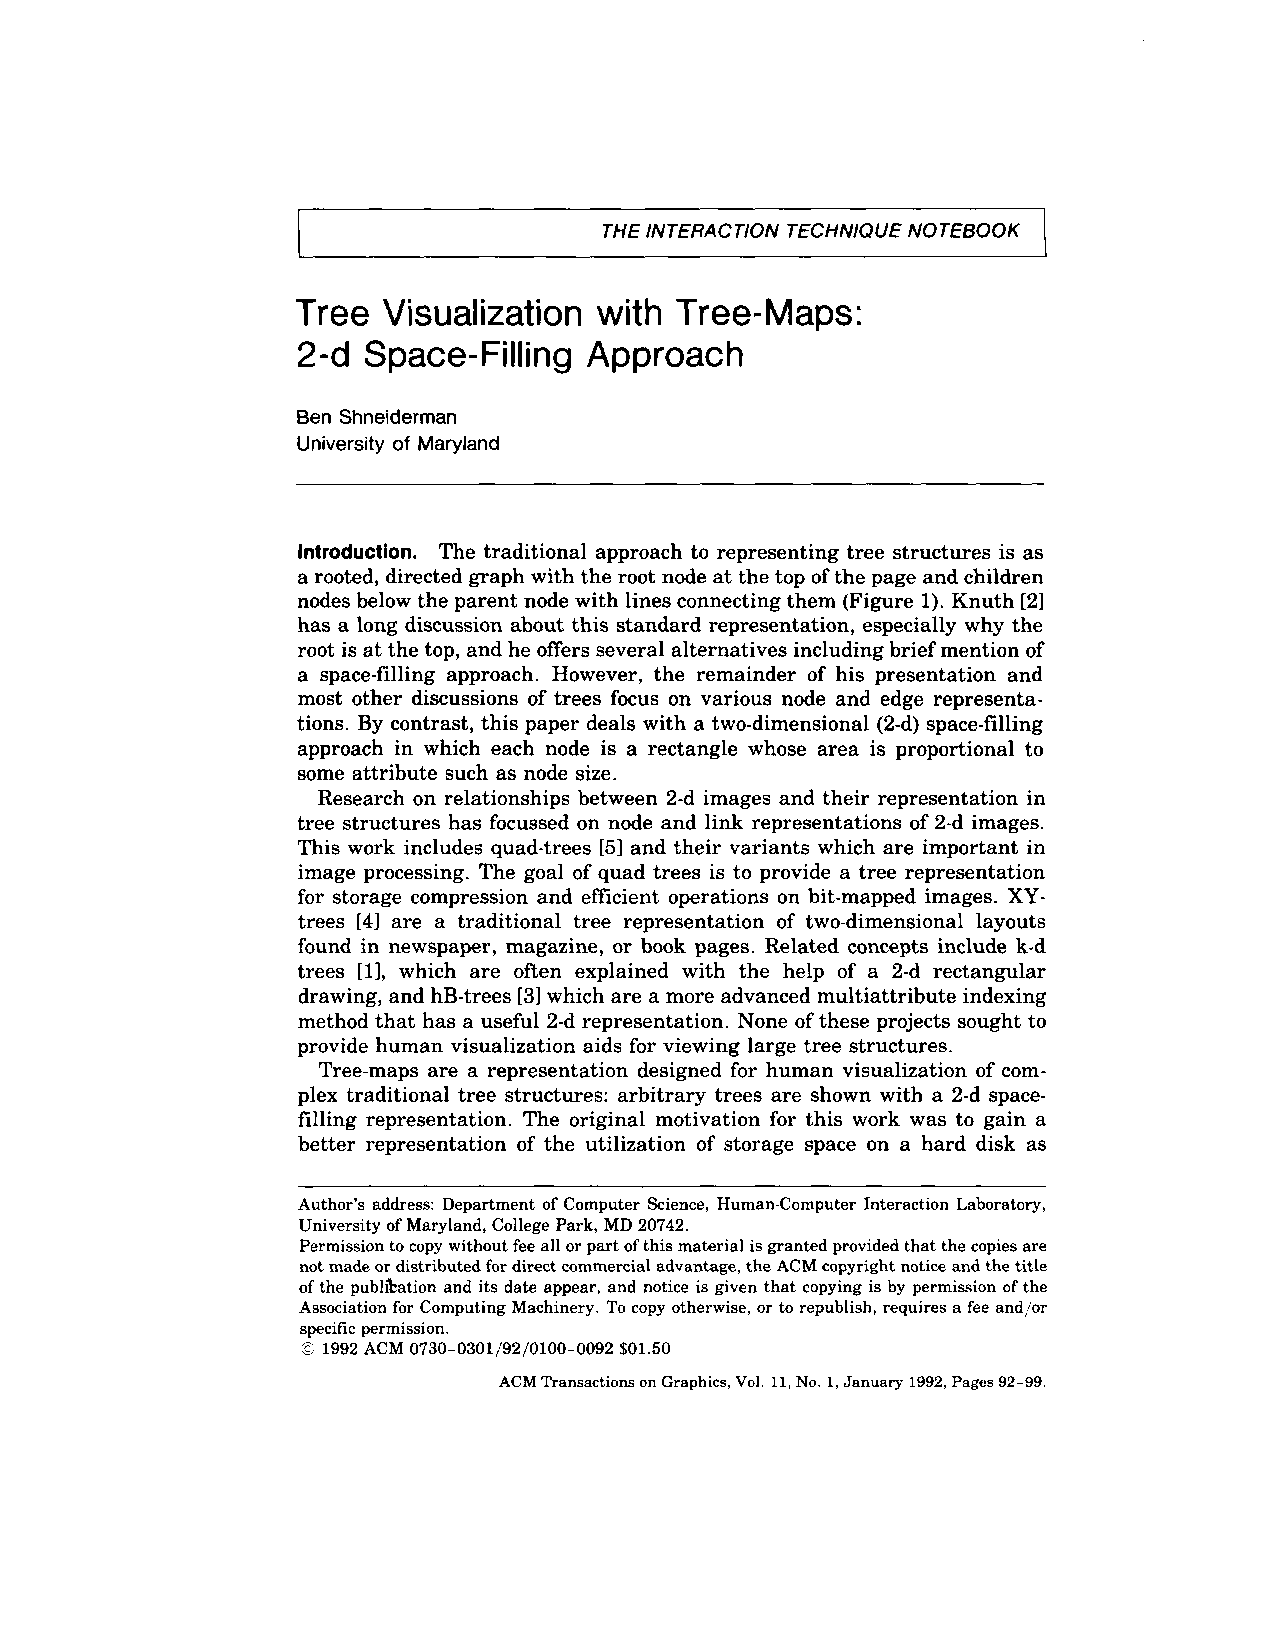
\includegraphics[height=10cm]{includes/SliceAndDice}
    \caption{Treemap - Slice-And-Dice-Algorithmus}
    \label{fig:sliceAndDice}
\end{figure}

\subsection*{Squarified Treemaps}

\begin{figure}[ht]
    \centering
    \includegraphics[height=10cm]{includes/SquarifiedTreemaps}
    \caption{Squarified Treemap}
    \label{fig:squarifiedTreemap}
\end{figure}

\begin{figure}[ht]
    \centering
    \includegraphics[height=10cm]{includes/SquarifiedTreemaps2}
    \caption{Squarified Treemap - absteigende Reihenfolge}
    \label{fig:squarifiedTreemap2}
\end{figure}

\subsection*{Vergleich}

\section{Aufgabe 4.2 | DNS-Vergleich mit Dendroscope}
\subsection*{XXX}

\end{document}
